\renewcommand{\theequation}{\theenumi}
\begin{enumerate}[label=\arabic*.,ref=\thesubsection.\theenumi]
\numberwithin{equation}{enumi}
\item given that $\to$
\\
No of experiment = 1000
\\
No of heads = 455
\\
No of tails = 545
\\
probability of comming heads = P$\left(X=0\right)$
\\
\begin{align}
P\left(X=0\right) &= \frac{455}{1000}
\\
&= 0.45
\end{align}
\item probability of comming Tails = P$\left(X=1\right)$
\\
\begin{align}
 P\left(X=1\right) &= \frac{545}{1000}
\\
&= 0.545
\end{align}
codes for the above equation can be get from here
\begin{lstlisting}
codes/probexm/probexm1.py
\end{lstlisting}
\begin{figure}[!ht]
	\centering
	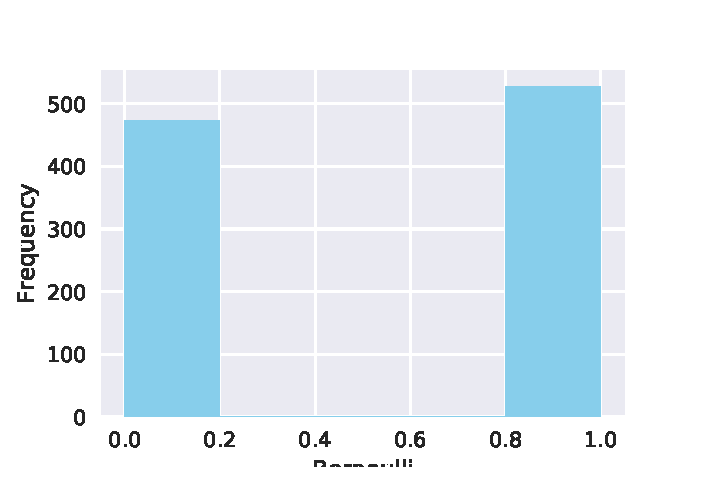
\includegraphics[width=\columnwidth]{./figures/probexm/probexm1.eps}
	\caption{bernoulli distribution of cointo be head}
	\label{fig:bt2}
	\begin{lstlisting}
	figs/probexm/probexm1.eps
	\end{lstlisting}
\end{figure}
\end{enumerate}